\subsection{第 17 课 | 布隆过滤器和LRU缓存}

\subsubsection{脑图}

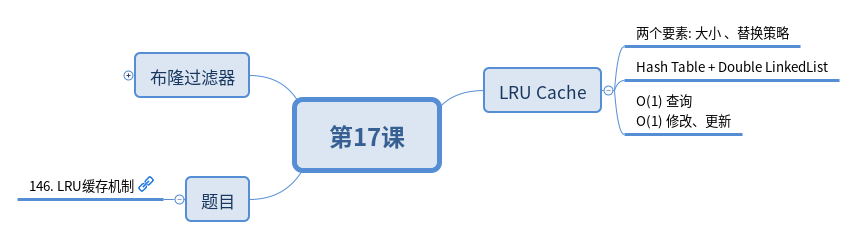
\includegraphics[width=150mm,height=40mm]{images/camp/第17课.png}

\subsubsection{题目}

\begin{itemize}
  \item \hyperref[leetcode:146]{146. LRU缓存机制}
\end{itemize}

\subsubsection{扩展阅读}

\href{https://www.cnblogs.com/cpselvis/p/6265825.html}{布隆过滤器的原理和实现} \\
\href{https://blog.csdn.net/tianyaleixiaowu/article/details/74721877}{使用布隆过滤器解决缓存击穿、垃圾邮件识别、集合判重} \\
\href{https://github.com/jhgg/pybloof}{高性能布隆过滤器 Python 实现示例} \\
\href{https://github.com/lovasoa/bloomfilter/blob/master/src/main/java/BloomFilter.java}{布隆过滤器 Java 实现示例 1} \\
\href{https://github.com/Baqend/Orestes-Bloomfilter}{布隆过滤器 Java 实现示例 2}

\href{https://www.sqlpassion.at/archive/2018/01/06/understanding-the-meltdown-exploit-in-my-own-simple-words/}{Understanding the Meltdown exploit} \\
\href{https://en.wikipedia.org/wiki/Cache_replacement_policies}{替换算法总揽} \\
